Es gibt verschiedene Möglichkeiten das magnetische Moment zu messen. In diesem Versuch wird die Hochfrequenzmethode verwendet, die in diesem Kapitel erklärt wird. Danach wird der gesamte Aufbau des Experiments und die Durchführung der Messung beschrieben.

\subsection{Hochfrequenz-Methode}
Die Hochfrequenz-Methode basiert auf der Aufspaltung der Energieniveaus, wenn ein magnetisches Moment in ein Magnetfeld gebracht wird. Es entstehen für Elektronen (Spin~$\frac{1}{2}$) zwei Zustände, wobei der Zustand mit niedrigerer Energie $E_0$ im thermodynamischen Gleichgewicht bei Raumtemperatur stärker besetzt ist als der Zustand mit der höheren Energie $E_1$. Elektronen können durch Energiezufuhr von $E_0$ in $E_1$ gebracht werden. Die Energie wird durch eine elektromagnetisches Feld bereitgestellt. Damit ein Übergang möglich ist, müssen das Magnetfeld und die Frequenz $\nu$ des elektromagnetischen Feldes aufeinander abgestimmt sein, sodass die Resonanzbedingung 
\begin{equation}
	\Delta E = \textrm{h} \nu = g \mu_\textrm{B} B
\end{equation}
erfüllt ist (siehe Abb. \ref{fig:elektron} ). Dabei klappen die Spins um. \\
Für Magnetfelder mit einer Stärke von einigen \si{\milli\tesla} liegt die Resonanzfrequenz im hochfrequenten Bereich mit ungefähr \SI{100}{\mega\hertz} und für Felder mit der Magnetfeldstärke einiger \si{\tesla} im Mikrowellen Bereich.
\\
\begin{figure}[h!]
	\centering
	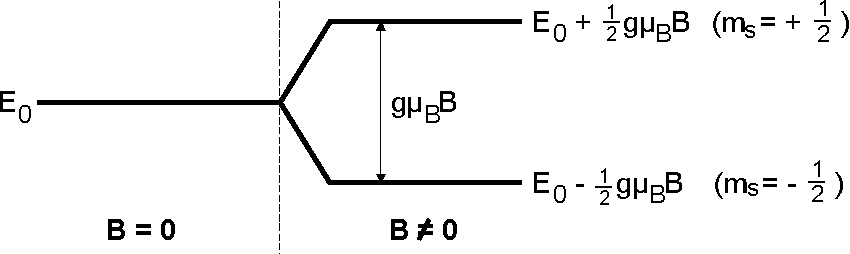
\includegraphics[width=0.6\textwidth]{Anleitung_Abb6.pdf}
	\caption{Energieniveaus  des Elektrons \cite{V28}}
	\label{fig:elektron}
\end{figure}

\subsection{Aufbau des Versuchs}

\subsection{Messung}
Es werden für fünf verschiedene Frequenzen die Resonanzen gemessen, indem die Stärke des Magnetfeldes variiert wird. Um optimale Messergebnisse zu erzielen müssen für jede Messung die Geräte aufeinander abgestimmt werden. Wichtig ist, dass beim Einstellen immer globale Extrema gesucht werden.

\begin{enumerate}
	
\item{Der gewünschte \textbf{Frequenzbereich} wird ausgewählt und die Geräte darauf eingestellt.}

\item{Die Frequenz des \textbf{Überlagerungssignals} wird so eingestellt, dass sie zirka um \si{552}{\kilo\hertz} von der Eingangsfrequenz abweicht. Das Ausgangssignal soll so groß wie möglich sein.}

\item{Die \textbf{Brückenschlatung} wird zunächst über die Einstellung $C_\textrm{grob}$ und dann über $C_\textrm{fein}$ und $R_\textrm{Abgleich}$ so angepasst, dass das Ausgangssignal minimiert wird. Der Signalverstärker muss ausgeschaltet sein. Dazu wird bei einem Wert des Ausgangssignals von knapp über \si{0,065}{\volt}  der Verstärker so eingestellt, dass die Spannung wieder ein Maximum einnimmt. Minimiert wird dann wieder mit Hilfe des Einstellungen von $C_\textrm{fein}$ und $R_{\textrm{Abgleich}}$.}

\item{Um die charakteristische \textbf{Lorentz-Kurve} (siehe Abb. \ref{fig:kurve}) zu erhalten, muss das Ausgangssignal ein wenig erhöht werden durch die Veränderung von $R_\textrm{Abgleich}$.}

\item{Der \textbf{X-Y-Schreiber} wird so eingestellt, dass es die Kurve komplett aufnimmt.}
\item{Der X-Y-Schreiber wird für jede Messung einzeln kalibriert, indem für fünf Werte in X-Richtung die Stromstärke notiert wird.}

\end{enumerate}


\begin{figure}[h!]
	\centering
	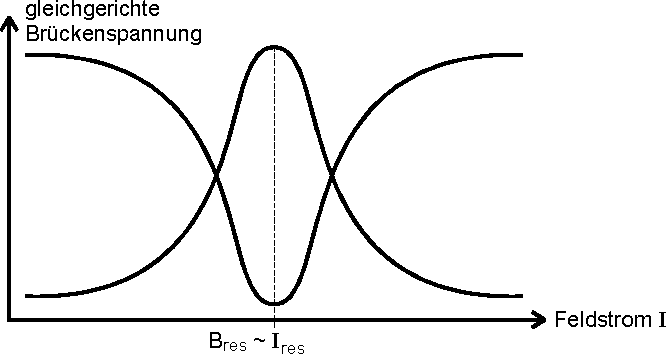
\includegraphics[width=0.6\textwidth]{Anleitung_Abb10.pdf}
	\caption[Resonanzkurve]{Gesuchte Resonanzkurve (Lorentz-Kurve) \cite{V28}}
	\label{fig:kurve}
\end{figure}
